% Capítulo 3
\chapter{Merge Sort}

\section{Gráfico}
O gráfico abaixo representa o tempo de execução esperado do merge-sort em função do tamanho da entrada. Como entrada para gerar o gráfico, foram utilizados 91 vetores de tamanho n, preenchidos com números gerados aleatoriamente de 0 até n. Pela análise do gráfico podemos notar que o algoritmo, desconsiderando a variação de tempo gerada por processos concorrentes no momento da execução do programa, pertence a O(n*log(n)).

O merge-sort nâo apresenta distinção de tempo dependendo da entrada, portanto, seu tempo é consistente e nâo pode ser análisado por melhor, pior e médio caso.
\begin{figure}[h]
    \centering
    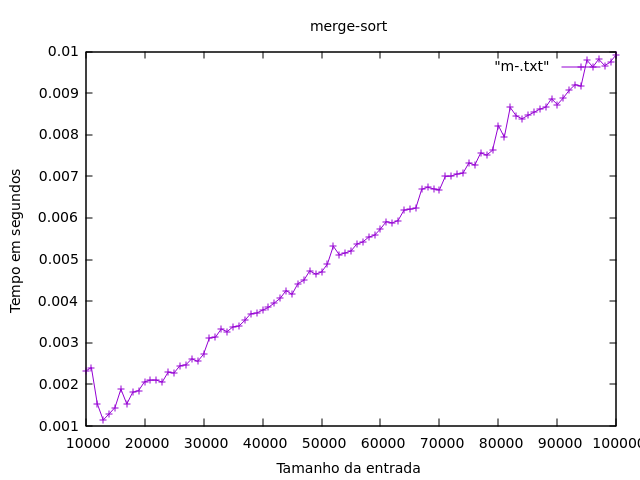
\includegraphics[width=1\linewidth]{Imagens/m-.png}
\end{figure}

\newpage

\section{Análise analítica do tempo de execução}

\subsection{Algoritmo}
\begin{figure}[h]
    \centering
    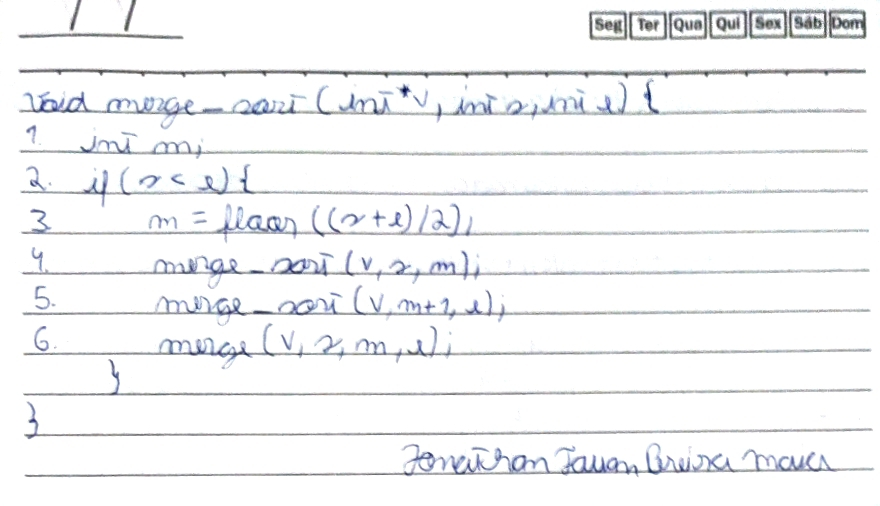
\includegraphics[width=0.76\linewidth]{Imagens/merge.jpg}
\end{figure}

\newpage
\subsubsection{Tempo esperado}
A análise analítica do tempo de execução do merge-sort permitiu perceber que em todos os casos o seu tempo de execução será sempre (n*log (n)).
\begin{figure}[h]
    \centering
    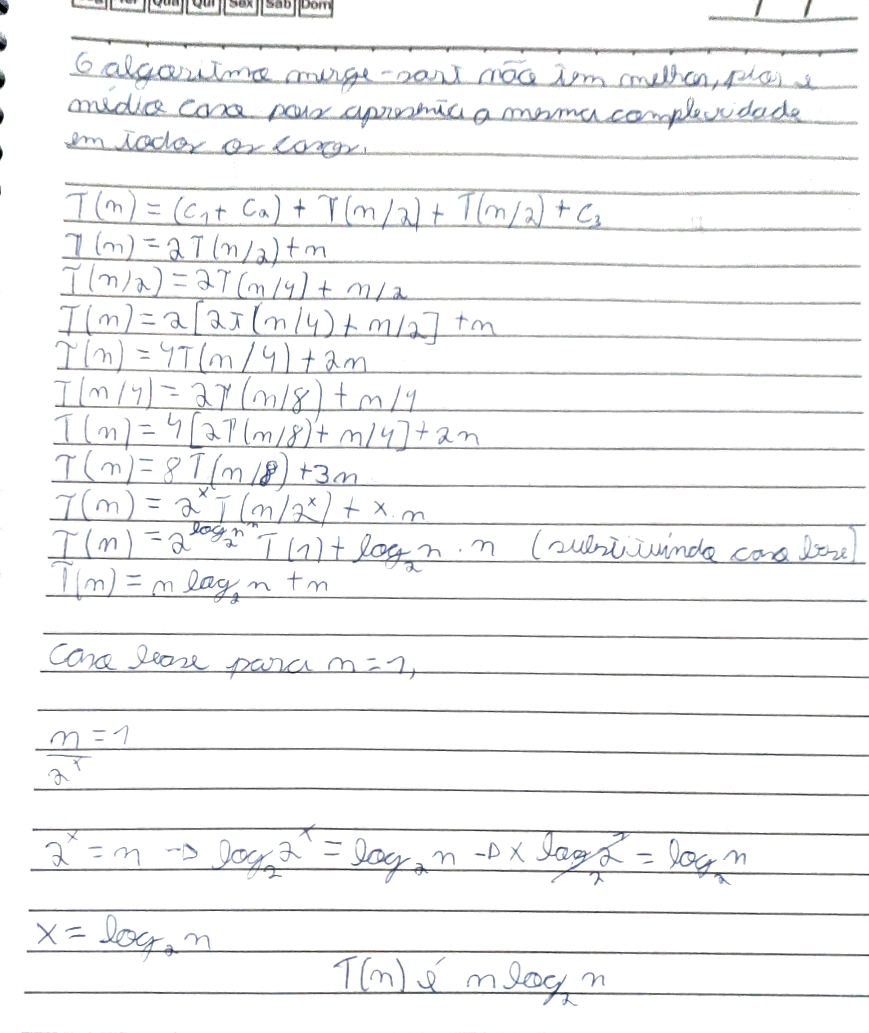
\includegraphics[width=0.76\linewidth]{Imagens/calculo-merge.jpg}
\end{figure}